% CVPR 2022 Paper Template
% based on the CVPR template provided by Ming-Ming Cheng (https://github.com/MCG-NKU/CVPR_Template)
% modified and extended by Stefan Roth (stefan.roth@NOSPAMtu-darmstadt.de)

\documentclass[10pt,twocolumn,letterpaper]{article}

%%%%%%%%% PAPER TYPE  - PLEASE UPDATE FOR FINAL VERSION
%\usepackage[review]{cvpr}      % To produce the REVIEW version
\usepackage{cvpr}              % To produce the CAMERA-READY version
%\usepackage[pagenumbers]{cvpr} % To force page numbers, e.g. for an arXiv version

% Include other packages here, before hyperref.
\usepackage{graphicx}
\usepackage{amsmath}
\usepackage{amssymb}
\usepackage{booktabs}


% It is strongly recommended to use hyperref, especially for the review version.
% hyperref with option pagebackref eases the reviewers' job.
% Please disable hyperref *only* if you encounter grave issues, e.g. with the
% file validation for the camera-ready version.
%
% If you comment hyperref and then uncomment it, you should delete
% ReviewTempalte.aux before re-running LaTeX.
% (Or just hit 'q' on the first LaTeX run, let it finish, and you
%  should be clear).
\usepackage[pagebackref,breaklinks,colorlinks]{hyperref}


% Support for easy cross-referencing
\usepackage[capitalize]{cleveref}
\crefname{section}{Sec.}{Secs.}
\Crefname{section}{Section}{Sections}
\Crefname{table}{Table}{Tables}
\crefname{table}{Tab.}{Tabs.}


%%%%%%%%% PAPER ID  - PLEASE UPDATE
\def\cvprPaperID{*****} % *** Enter the CVPR Paper ID here
\def\confName{CVPR}
\def\confYear{2022}

\graphicspath{{./figures/}}
\begin{document}

%%%%%%%%% TITLE
\title{Generating Expressive Facial Mesh Animation : A Survey}

\author{
HJW\\
Institution1 address\\
{\tt\small self@yukinyaa.moe}
% For a paper whose authors are all at the same institution,
% omit the following lines up until the closing ``}''.
% Additional authors and addresses can be added with ``\and'',
% just like the second author.
% To save space, use either the email address or home page, not both
}
\maketitle

%%%%%%%%% ABSTRACT
\begin{abstract}
With technology allowing for increasing realism in games and movies, facial animation is still a very challenging task. 

"Lorem ipsum dolor sit amet, consectetur adipiscing elit, sed do eiusmod tempor incididunt ut labore et dolore magna aliqua. Ut enim ad minim veniam, quis nostrud exercitation ullamco laboris nisi ut aliquip ex ea commodo consequat. Duis aute irure dolor in reprehenderit in voluptate velit esse cillum dolore eu fugiat nulla pariatur. Excepteur sint occaecat cupidatat non proident, sunt in culpa qui officia deserunt mollit anim id est laborum."
\end{abstract}

%%%%%%%%% BODY TEXT
\section{Introduction}
\label{sec:intro}

Human tend to be very sensitive to facial motion psychologically. Slightest uncanniest in facial animation directly leads to hurt overall experience\cite{hansonUpendingUncannyValley}. Facial animation can be applied to multiple applications such as computer games, e-commerce, immersive VR telepresence, and movies. Yet achieving realistic facial animation is a challenging task. So, delivering natural expressive facial animation is a great interest in graphics field.

Animating high-quality expressive face is very labor-intensive job when done by animator. Another approach to animate face is to capture human face animation in 3D. Face capture is a well-understood field(cite here), yet such approach requires gigabytes of data from expensive capture system, and is hard to manipulate. Therefore, it is necessary to simplify such process. 

To simplify such process, one can automatically generate facial animation or can simplify animating produce.

In this survey, I introduce and compare three research that animate expressive facial animation :
\begin{itemize}
 \item JALI\cite{edwardsJALIAnimatorcentricViseme2016} and VisimeNet\cite{zhouVisemenetAudiodrivenAnimatorcentric2018}, a linguistic approach to lip-sync.
 \item MeshTalk\cite{richardMeshTalk3DFace2021}, a deep learning method.
 \item D3DExpression\cite{potamiasLearningGenerateCustomized2020}, LSTM method which replicate facial expression.
\end{itemize}


% Creating lip-sync animation is complex and challenging task.
% Mapping face expression to latent space is actively being researched due to recent advancement in deep learning field.



\section{Methods}

\subsection{JALI and Visemenet}

\subsubsection{JALI}

\begin{figure}
   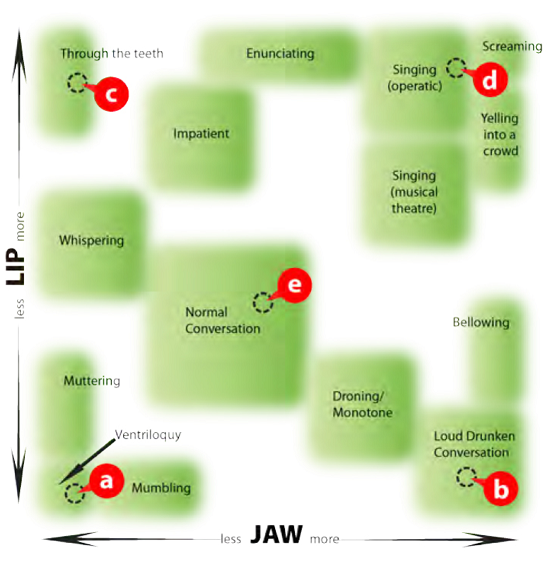
\includegraphics[width=1.0\linewidth]{jaliStyles}
   
   \caption{Speaking styles of JALI viseme field}
   \label{fig:jaliStyles}
\end{figure}

%Introducing: a linguistic approach, an old approach
Lip-sync can be done by linguistic approach which is mapping text to phonemes, then phonemes to visemes\cite{ezzatMikeTalkTalkingFacial1998}. Viseme is a specific facial shape when making certain sound. A traditional facial rig can have many-to-one mapping from phonemes to visemes, or many-to-many using dynamic visemes. This approach can achieve realistic acoustic motion on the model.

%Introduce JALI
JALI\cite{edwardsJALIAnimatorcentricViseme2016} is a state-of-the-art viseme model that can generate lip-sync animation from English text and voice. JALI takes jaw and lip activation multipliers into consideration, since jaw and lip is the most significant acoustic motion in face. As shown on \cref{fig:jaliStyles}, different speaking styles shows different jaw lip activation level multipliers, which can be animated more intuitively.

%about linguistic model, suppressor rules etc
JALI use text-to-phoneme speech library built in to OSX. This converts English text into a phonemic representation. Next, text is forced aligned, which is a process that aligning phonemes to text. Audio must be annotated with the beginning, middle, and end of each phoneme. This is typically done by training Hidden Markov Model. Several tools exist for this task such as HTK and SPHINX.

JALI animates a facial rig by producing sparse animation keyframes for visemes, by some linguistic rules. When animating, lexical stress and co-articulation rule is considered. Co-articulation is a rule which visemes interact with each other. For example, duplicated visemes such as /p/ and /m/ in "pop man" are co-articulated into one MMM viseme, and tongue-only visemes have no influence on the lips, and lip takes shape of the surrounding visemes.

%Volume of each word have to be considered to determine which word is stressed. It is impossible to determine volume of plosive (e.g. p b d) or fricative (e.g. s z f). But vowel (a e i o u) is always voiced, so stress can be easily determined.

%Strength of JALI
Unlike other methods, JALI can produce sparse keyframed procedural animation. Generated animation can be edited to achieve more idiosyncratic animation. It is also easy to accompany the method with other animation, since animation only affects jaw and lip parameter of the rig.

%Limitation of JALI
Limitation of the work is that it lacks some auditory parameter such as rate of speech, and jitter and shimmer. Also, emotional speech styles are not considered. Emotional styles can affect subtle parameter, but is a critical part of expressiveness of the animation.

\subsubsection{Visemenet}

\begin{figure*}
   \centering
   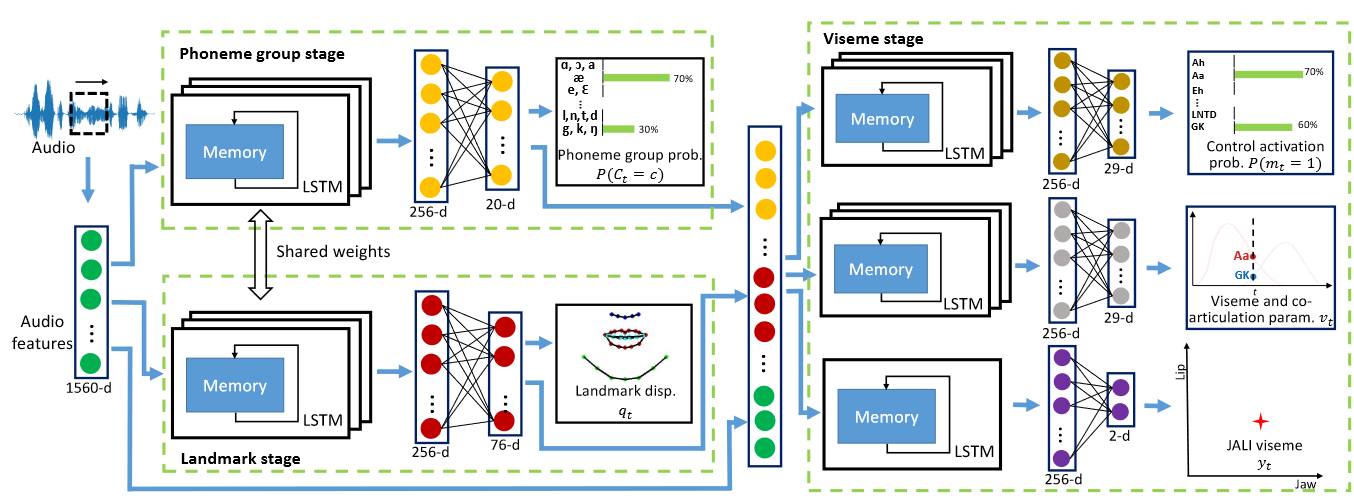
\includegraphics[width=1.0\linewidth]{VisemenetArchitecture}
   \caption{Architecture of Visemenet model.}
   \label{fig:VisemenetArchitecture}
\end{figure*}


%Significance of Audio to animation.

%Introdude Visemenet
Visemenet is a deep-learning based lip-sync method based on JALI model. Unlike JALI, Visemenet takes auditory data only to generate JALI lip-sync animation. Visemenet tries to replicate linguistic model with multiple deep-learning LSTM layers.

%network overview
As shown on \cref{fig:VisemenetArchitecture}, Visemenet mainly have three stages. Phoneme group stage, landmark stage, and viseme stage. Phoneme and landmark stage is a pretrained model with relatively large amount of dataset, and Viseme stage a main model which predicts three types of JALI animation parameters.

%Pretrain network And datastet
Auditory data is converted to multiple features that has been used in previous studies. 65 feature vectors of 3 type per each frame is used, and 24 frames are used as input of all network, sum 1560 dimension.

Phoneme groups are 20 groups of phonemes which corresponds to certain visemes. Phoneme group stage estimates phoneme group from audio features.

38 artist-defined landmarks in real face with jaw, lip and nose is considered in landmark stage. Landmark stage estimates 2D-displacement of this landmark, resulting in 76 dimension output.

Pretrain networks are trained with about total 15 hour worth of publically available audiovisual facial dataset. Dataset used in training must have English transcript and corresponding voiced video. Most of the video dataset available used for facial recognition has transcript and high quality video recorded with camera at front of the face.

%Main network And dataset
Viseme stage is a main network that predicts JALI model variables. Input of the network is 1560 dimension audio features and 20 dimension predicted phoneme groups, and 76d landmark displacement groups. JALI control activation and visemes, co-articulation parameters are predicted in individual LSTM networks. LSTM layers have 256-dimension memory state, with 2 fully connected decoders.

Viseme stage is trained with 1 hour of rig motion curves. Experienced animator created dataset corresponding audio.

%Pros of Visemenet
Visemenet successfully mapped audio to speech motion curve. Pretrained network used hand-engineered audio features, replacing such features with learned feature will improve performance, which is happening at image processing.

%Limitation of Visemenet
This research mixes animator-centric technique and deep-learning method. But unlike JALI that shares low-dimension output, Visemenet generates frame-by-frame animation, which is harder to manipulate.

\subsection{MeshTalk}

\begin{figure}[t]
   \begin{center}
   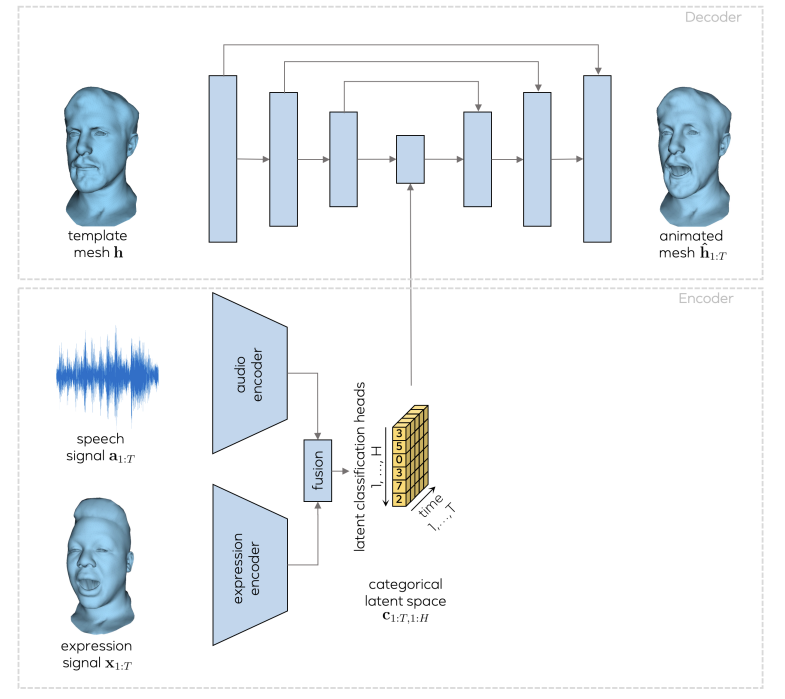
\includegraphics[width=0.8\linewidth]{meshtalk_overview.png}
   \end{center}
   \caption{The network diagram\cite{richardMeshTalk3DFace2021}.}
   \label{fig:long}
   \label{fig:networkdiag}
 \end{figure}

%Introduce Meshtalk
MeshTalk is a generic method for generating full facial mesh animation from speech. MeshTalk network can generate lip-sync animation from a single frame of generic human facial mesh and audio signal, and also can in expressive data from mesh animation.

%network overview
The network resembles Variational Autoencoder with multiple latent space as shown in Figure \ref{fig:networkdiag}.
Target mesh \(\hat{h}\) is estimated from template mesh \(h\) and latent space \(\mathsf{c}\) by computing function \(\mathcal{D}\).
\begin{equation}
  \hat{h}_{1:T} = \mathcal{D}(h, \mathsf{c}_{1:T, 1:H})
  \label{eq:1}
\end{equation}
Sequence of latent space \(\mathsf{c}_{1:T}\) is derived from audio sequence \(\mathsf{a}_{1:T}\) and expression signal mesh sequence \(\mathsf{x}_{1:T}\).
\(c\) and \(a\) are first mapped to \(T*H*C\) dimensional latent space, then passed through Gumbel-softmax\cite{jangCategoricalReparameterizationGumbelSoftmax2017} over every classification head.

%Mesh Data
%Pros of MeshTalk
%Limitation of MeshTalk

\subsection{D3DExpression}
%Introduction 
%network overview
%Overview
%Speech Data
%Mesh Data
%Pros of D3DExpression
%Limitation of D3DExpression

\subsection{Discussion}

\begin{table*}
   \centering
   \begin{tabular}{c|cc}
      \toprule
      Method & Input & Output \\
      \midrule
      JALI & Audio, transcript & JALI rigged keyframed lip-sync animation \\
      Visemenet & Audio & JALI rigged lip-sync animation \\
      MeshTalk & Audio, Expression mesh animation & Mesh animation\\
      D3DExpression & ?? & ??\\
      \bottomrule
   \end{tabular}
   \caption{Comparison of input and output of each method}
   \label{table:io_cmp}
\end{table*}


\begin{table*}
   \centering
   \begin{tabular}{c|cc}
      \toprule
      Method & Types & Data(in time) \\
      \midrule
      JALI & No training data & - \\
      Visemenet & Publically available Audio, Transcript, Video & 15h pretrain 1h main \\
      MeshTalk & In-house Audio, Mesh animation & 13h \\
      D3DExpression & ?? & ??\\
      \bottomrule
   \end{tabular}
   \caption{Comparison of traning dataset of each method}
   \label{table:data_cmp}
\end{table*}
%compare input and output with sheet

%compare training data with sheet

%%%%%%%%% REFERENCES
{\small
\bibliographystyle{ieee_fullname}

\bibliography{refs}
}

\end{document}
